\documentclass[conference]{IEEEtran}
\IEEEoverridecommandlockouts

\usepackage{cite}
\usepackage{amsmath,amssymb,amsfonts}
\usepackage{algorithmic}
\usepackage{graphicx}
\usepackage{booktabs}
\usepackage{multirow}
\usepackage{subcaption}
\usepackage{url}
\usepackage{xcolor}

\def\BibTeX{{\rm B\kern-.05em{\sc i\kern-.025em b}\kern-.08em
    T\kern-.1667em\lower.7ex\hbox{E}\kern-.125emX}}

\begin{document}

\title{
A Hierarchical Multimodal Framework for Autonomous Maritime Surveillance Using Satellite Detection, Kalman-Filter UAV Tracking, and Vision-Language Reasoning
}

\author{
\IEEEauthorblockN{Aman Reddy J}
\IEEEauthorblockA{\textit{Department of Computer Science and Engineering} \\
\textit{Amrita School of Computing, Amrita Vishwa Vidyapeetham} \\
Chennai, India \\
amanreddyjukonti@gmail.com}
\and
\IEEEauthorblockN{BTPR Nikhil}
\IEEEauthorblockA{\textit{Department of Computer Science and Engineering} \\
\textit{Amrita School of Computing, Amrita Vishwa Vidyapeetham} \\
Chennai, India \\
btprnikhil@gmail.com}
}

\maketitle

\begin{abstract}
Persistent maritime domain awareness requires bridging strategic wide-area observation with tactical localized inspection under severe edge-compute and bandwidth constraints. This paper presents OATrack-VLM, an end-to-end hierarchical multimodal framework that unifies high-resolution satellite vessel detection, tactical UAV tracking via a discrete linear Kalman filter, fine-grained vessel classification, reinforcement-learning-driven adaptive compute scheduling, and vision-language reasoning. Strategic wide-area surveillance employs a fine-tuned YOLO11n detector operating at high input resolution ($1024\times1024$), achieving 93.64\% precision, 90.26\% recall, and 94.63\% mAP@50 on the VHRV optical satellite benchmark. Detected target coordinates are handed off to a tactical UAV surveillance stage, where an 8-state linear Kalman filter tracking pipeline maintains persistent vessel identities across occlusions, scale shifts, and temporary detector dropouts through multi-feature association and sub-part suppression. Cropped vessel targets are categorized across ten maritime classes using ConvNeXt-Tiny (81.56\% top-1 accuracy, 82.84\% macro F1), reinforced by temporal evidence aggregation across track lifetimes. To mitigate edge energy expenditure during long-endurance patrols, an integrated Gymnasium-trained Proximal Policy Optimization (PPO) scheduler dynamically throttles frame processing, yielding estimated compute reductions of 75.00\% on quiescent waters and 45.46\%--52.12\% on active naval sequences while safeguarding tracking continuity via an operational safety override. Finally, a grounded vision-language reasoning layer synthesizes telemetry-verified tactical intelligence briefings without ungrounded hallucinations. The unified system bridges strategic monitoring and persistent tactical surveillance for resource-constrained aerial maritime operations.
\end{abstract}

\begin{IEEEkeywords}
Maritime surveillance, satellite detection, UAV tracking, Kalman filter, vessel classification, adaptive edge computing, reinforcement learning, vision-language models.
\end{IEEEkeywords}

\section{Introduction}

Maritime domain awareness is vital for national defense, territorial border protection, exclusive economic zone (EEZ) enforcement, fisheries protection, and search-and-rescue operations across expansive oceanic theaters~\cite{pohontu2024}. Conventional maritime monitoring architectures predominantly rely on optical or synthetic aperture radar (SAR) satellite imagery for wide-area spatial coverage. While satellite remote sensing excels at detecting surface targets across vast oceanic expanses, orbital revisit intervals and orbital mechanics preclude continuous, persistent observation of dynamic vessels. Conversely, tactical unmanned aerial vehicles (UAVs) provide low-altitude maneuverability, high-resolution continuous video observation, and agile camera angles. However, deploying UAVs to blindly search thousands of square kilometers of open ocean without prior spatial cues leads to rapid battery depletion, limited coverage, and missed detections.

Recent research has introduced deep neural networks for automated vessel detection and classification from remote sensing and aerial platforms~\cite{tang2024,sun2021,yu2024,ren2026,kizilkaya2025}. Nevertheless, these operational stages have largely evolved as disjoint technologies. Satellite detection frameworks rarely interface seamlessly with aerial tracking pipelines; tracking systems frequently suffer from track fragmentation and identity switching under temporary occlusion, wave spray, or scale variation; and downstream intelligence generation typically requires human analysts to interpret raw bounding boxes and classification labels. Moreover, running continuous high-resolution object detection and deep convolutional neural networks at full frame rates on edge-constrained drone platforms quickly exhausts available power budgets, severely curtailing flight endurance.

To overcome these structural limitations, this paper proposes OATrack-VLM, an integrated hierarchical multimodal framework for autonomous maritime surveillance. As illustrated in Fig.~\ref{fig:system_architecture}, the proposed architecture organizes perception across strategic, tactical, and semantic reasoning tiers:
\begin{enumerate}
    \item \textbf{Strategic Satellite Localization:} High-resolution ($1024\times1024$) YOLO11n inference identifies candidate vessels across wide-area optical satellite scenes, suppressing downsampling truncation of small vessels.
    \item \textbf{Target Handoff Adapter:} Verified satellite vessel coordinates seed localized tactical UAV flight paths, eliminating wasteful open-ocean transit searches.
    \item \textbf{Kalman-Filter UAV Tracking:} An 8-dimensional discrete linear Kalman filter integrates constant-velocity motion and scale prediction, two-stage multi-feature data association, and sub-part suppression to maintain continuous track persistence across temporary missed detections.
    \item \textbf{Fine-Grained Classification \& Evidence Aggregation:} Context-expanded vessel crops are classified across ten distinct maritime categories using ConvNeXt-Tiny, with multi-frame probability aggregation stabilizing classifications against transient viewpoint fluctuations.
    \item \textbf{PPO Adaptive Edge Compute Scheduling:} A Proximal Policy Optimization (PPO) policy running in an edge Gymnasium environment dynamically modulates sampling intensity between lightweight, standard, and full tactical modes, reducing compute waste on empty waters while preserving responsiveness via an operational safety override.
    \item \textbf{Grounded Vision-Language Intelligence Synthesis:} A vision-language reasoning layer converts structured tracking telemetry and tactical visual crops into coherent intelligence briefings while enforcing strict grounding constraints against unsupported hallucinations.
\end{enumerate}

\begin{figure*}[t]
\centering
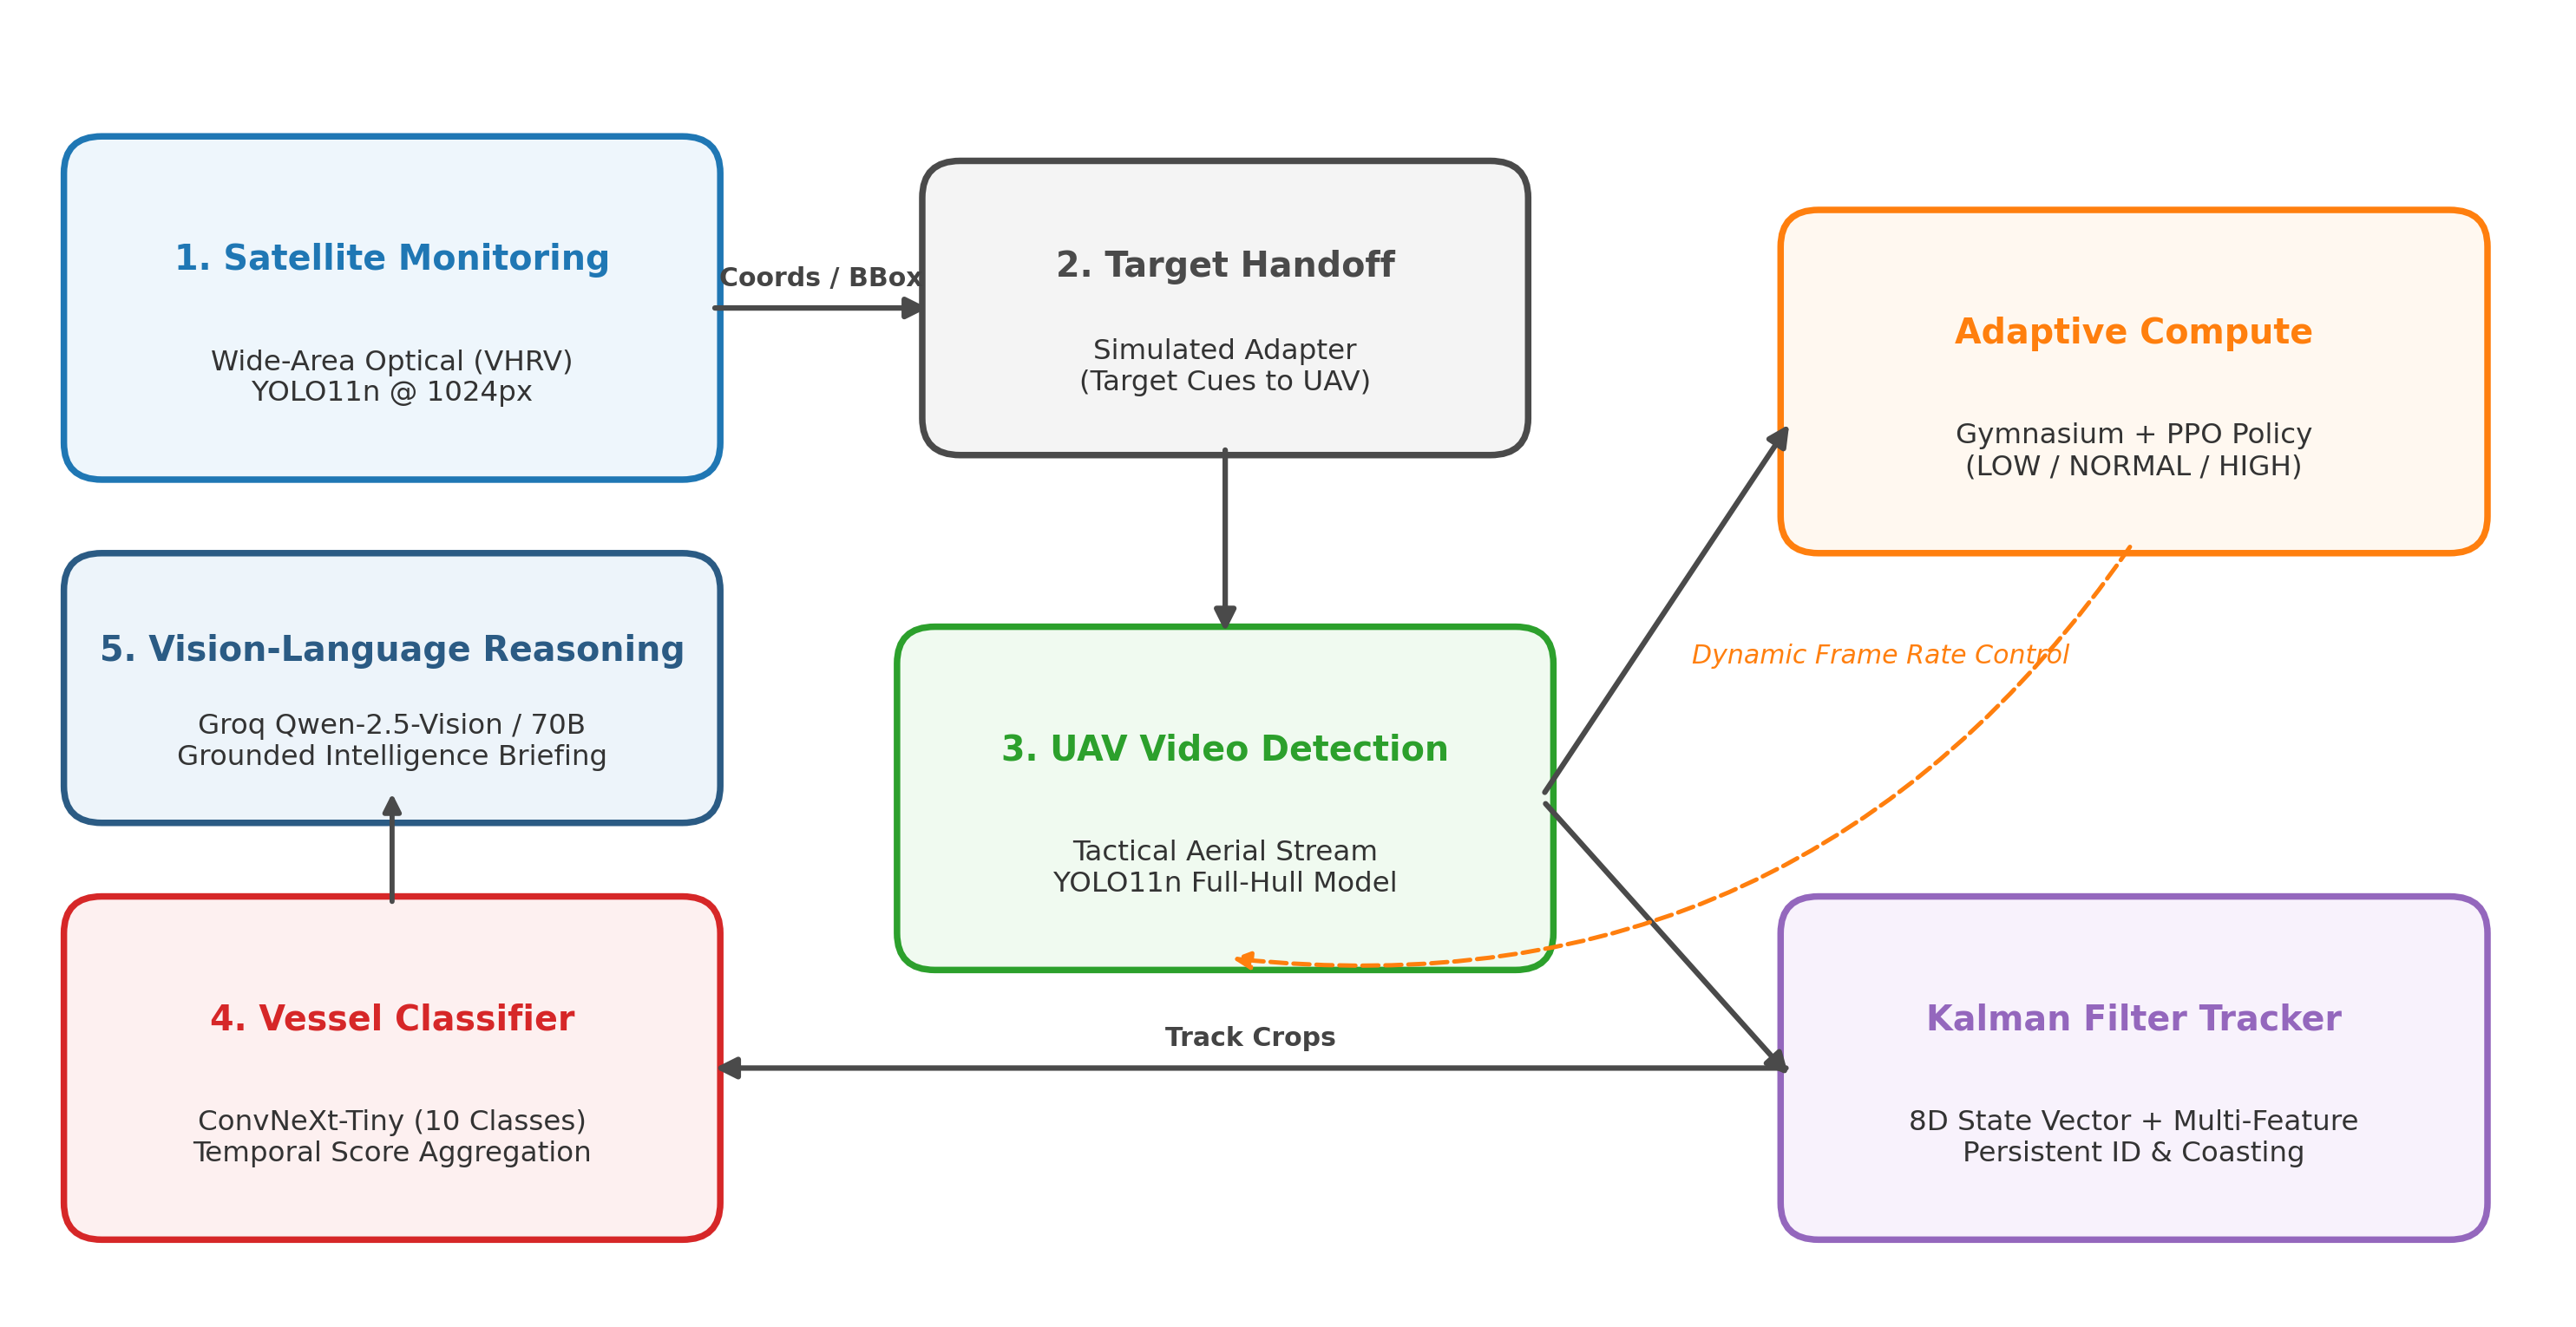
\includegraphics[width=0.98\textwidth]{figures/system_architecture.png}
\caption{End-to-end system architecture of the OATrack-VLM maritime surveillance framework, illustrating the hierarchical progression from strategic wide-area satellite monitoring to tactical UAV tracking, adaptive edge compute scheduling, fine-grained vessel classification, and grounded vision-language reasoning.}
\label{fig:system_architecture}
\end{figure*}

\section{Related Work}

\subsection{Maritime Vessel Detection from Satellite and Aerial Platforms}
Automated vessel detection from satellite and aerial remote sensing has advanced rapidly through convolutional neural network architectures. Tang et al.~\cite{tang2024} implemented an enhanced YOLOv7 architecture with specialized convolutions for SAR ship detection, while Sun et al.~\cite{sun2021} presented BiFA-YOLO for arbitrary-oriented vessel localization in SAR imagery. Yu and Shin~\cite{yu2024} utilized channel-shuffled reparameterized convolution blocks and dynamic heads to balance speed and accuracy in maritime detection. Ren et al.~\cite{ren2026} addressed dense harbor scenarios using multi-scale context extraction and feature enhancement. K{\i}z{\i}lkaya et al.~\cite{kizilkaya2025} developed the VHRShips benchmark to standardize evaluation on very-high-resolution optical satellite imagery. Additionally, Xiao et al.~\cite{xiao2026} demonstrated that YOLOv11n achieves competitive detection speeds on embedded hardware. However, these works focus almost exclusively on static single-image localization and do not investigate target handoff to mobile aerial platforms.

\subsection{Multi-Object Tracking and Kalman Filtering}
Multi-object tracking (MOT) in dynamic video feeds relies on the tracking-by-detection paradigm. The foundational Simple Online and Realtime Tracking (SORT) framework~\cite{bewley2016sort} demonstrated that an 8-state Kalman filter~\cite{kalman1960} coupled with the Hungarian association algorithm delivers high tracking throughput and stable short-term trajectory estimation. DeepSORT~\cite{wojke2017deepsort} incorporated deep appearance embeddings to reduce ID switching during long-term occlusions, albeit at substantial inference cost. ByteTrack~\cite{zhang2022bytetrack} introduced two-stage association, matching high-confidence detections first and subsequently pairing low-confidence detections with active tracks to recover occluded objects. While effective for terrestrial traffic and pedestrian tracking, aerial maritime surveillance presents distinct challenges: vessel bounding boxes exhibit dramatic scale variations depending on drone altitude, wake turbulence generates false positives, and close-quarter moorings cause single vessels to fragment into deck-fitting detections. The tracking component in this work designs an 8-state discrete Kalman filter with a multi-feature association metric incorporating bounding-box IoU, normalized centroid displacement, aspect-ratio similarity, and sub-part containment suppression.

\subsection{Fine-Grained Vessel Classification}
Fine-grained maritime vessel recognition is inherently challenging due to high intra-class variation (varying vessel paint schemes, cargo configurations, and antenna arrays) and low inter-class variation among naval combatants (such as Frigates, Destroyers, and Cruisers)~\cite{guo2026}. Liu et al.~\cite{liu2022convnet} introduced ConvNeXt, re-engineering standard convolutional networks with inverted bottlenecks and large kernels to match vision transformer accuracy with lower computational overhead. Guo et al.~\cite{guo2026} introduced IFShip, utilizing domain-specific prompt engineering and vision-language models for interpretable ship classification. While foundation vision models such as SAM~\cite{kirillov2023sam}, SAM~2~\cite{ravi2024sam2}, ALPS~\cite{zhang2025alps}, and Grounding DINO~\cite{liu2024groundingdino} exhibit strong open-set segmentation, their parameter footprint exceeds the real-time payload envelope of embedded UAV systems. In our framework, ConvNeXt-Tiny serves as an efficient edge classifier, reinforced by temporal evidence aggregation over persistent track observations.

\subsection{Adaptive Computing and Reinforcement Learning}
Deploying deep vision pipelines aboard power-constrained UAVs requires balancing detection accuracy against battery depletion. Li et al.~\cite{li2023drl} and Palmas~\cite{palmas2025} applied deep reinforcement learning to weapon-target assignment and drone defense prioritization. Schulman et al.~\cite{schulman2017ppo} developed Proximal Policy Optimization (PPO), which offers stable on-policy reinforcement learning across continuous and discrete control spaces. Luo et al.~\cite{luo2022} explored reinforcement learning for tactical resource allocation. In this work, PPO is leveraged to dynamically schedule edge inference frequency based on maritime scene complexity, vessel visibility, and tracking continuity, accompanied by a deterministic safety override layer.

\subsection{Vision-Language Models in Surveillance}
Recent advances in multimodal large language models have enabled automated video reasoning and situational awareness generation~\cite{desilva2024,feng2024}. However, unconstrained commercial VLMs are susceptible to hallucinating critical tactical attributes (e.g., vessel nationality, hull registration numbers, or unobservable armaments). In this framework, vision-language reasoning is grounded by passing verified detection bounding boxes, persistent track IDs, and classifier predictions directly within structured telemetry prompts, preventing ungrounded claims.

\section{System Overview}

The OATrack-VLM framework establishes a closed perception-to-intelligence loop connecting satellite remote sensing, aerial tracking, edge-compute scheduling, and tactical reporting:

\begin{equation}
I_{\text{sat}} \xrightarrow{\text{YOLO11n}} \mathcal{D}_{\text{vessel}} \xrightarrow{\text{Handoff}} \mathcal{T}_{\text{UAV}} \xrightarrow{\text{Kalman}} \mathcal{T}_{\text{id}} \xrightarrow{\text{ConvNeXt}} \mathcal{C}_{\text{stable}} \xrightarrow{\text{VLM}} \mathcal{R}_{\text{intel}}.
\end{equation}

Here, $I_{\text{sat}}$ denotes the optical satellite image, $\mathcal{D}_{\text{vessel}}$ represents satellite vessel bounding boxes, $\mathcal{T}_{\text{UAV}}$ denotes the tactical UAV video feed, $\mathcal{T}_{\text{id}}$ represents persistent tracks maintained by the Kalman filter, $\mathcal{C}_{\text{stable}}$ represents temporally aggregated vessel classifications, and $\mathcal{R}_{\text{intel}}$ denotes the generated natural-language intelligence briefing.

\section{Methodology}

\subsection{Satellite-Based Vessel Detection}
Very-high-resolution optical satellite imagery (typically $4800\times2886$ pixels in VHRV) exhibits extreme scale disparities: large container vessels span hundreds of pixels, while small fishing vessels collapse beneath convolutional feature strides if aggressively downsampled. To preserve spatial resolution without truncation, wide-area imagery is processed at $1024\times1024$ pixels through a fine-tuned YOLO11n detector. For each candidate vessel, the model outputs bounding-box coordinates $(x_1, y_1, x_2, y_2)$, confidence score $s \in [0, 1]$, and centroid $c_x = (x_1+x_2)/2$, $c_y = (y_1+y_2)/2$ with dimensions $w = x_2-x_1$, $h = y_2-y_1$. Non-maximum suppression with $\tau_{\text{conf}} = 0.25$ and $\tau_{\text{iou}} = 0.60$ filters low-confidence proposals and redundant overlaps.

\subsection{Target Handoff and Aerial UAV Detection}
Upon positive satellite detection, target coordinates and bounding geometries are packaged into a structured surveillance cue: $\mathcal{M}_{\text{handoff}} = \{N_{\text{vessels}}, \{(c_{x,i}, c_{y,i}, w_i, h_i, s_i)\}_{i=1}^{N_{\text{vessels}}}\}$. A software-in-the-loop simulation adapter seeds the tactical UAV flight path, eliminating open-ocean search transits. The UAV surveillance module ingests sequential video frames and executes localized vessel detection via a dedicated YOLO11n model calibrated for aerial perspectives ($\tau_{\text{drone}} = 0.18$, $\tau_{\text{iou}} = 0.45$), capturing full-hull bounds from bow to stern despite wake turbulence and sea spray.

\subsection{Kalman Filter-Based Vessel Tracking}
To preserve vessel identities across continuous drone surveillance feeds without ID switching, we formulate tracking as an 8-state discrete linear dynamical system. Each active track maintains state vector $\mathbf{x} = [c_x, c_y, w, h, v_x, v_y, v_w, v_h]^T \in \mathbb{R}^8$, modeling centroid coordinates, box dimensions, translational velocities $(v_x, v_y)$, and perspective scale evolution rates $(v_w, v_h)$. The measurement vector is $\mathbf{z} = [c_x, c_y, w, h]^T \in \mathbb{R}^4$.

Assuming a constant-velocity transition model with time step $\Delta t = 1$, the state transition matrix $\mathbf{F} \in \mathbb{R}^{8\times8}$ and measurement mapping $\mathbf{H} \in \mathbb{R}^{4\times8}$ are structured as block matrices $\mathbf{F} = [\mathbf{I}_4, \mathbf{I}_4; \mathbf{0}_4, \mathbf{I}_4]$ and $\mathbf{H} = [\mathbf{I}_4, \mathbf{0}_4]$. At frame $t$, state and covariance prediction are governed by:
\begin{equation}
\hat{\mathbf{x}}_t^- = \mathbf{F} \mathbf{x}_{t-1}, \quad \mathbf{P}_t^- = \mathbf{F} \mathbf{P}_{t-1} \mathbf{F}^T + \mathbf{Q},
\label{eq:kalman_pred}
\end{equation}
where $\mathbf{Q} = \text{diag}(\sigma_{p}^2, \sigma_{p}^2, \sigma_{p}^2, \sigma_{p}^2, \sigma_{v}^2, \sigma_{v}^2, \sigma_{s}^2, \sigma_{s}^2)$ models maneuver disturbances and camera jitter.

Upon associating measurement $\mathbf{z}_t$, the innovation residual and Kalman gain $\mathbf{K}_t$ update the state estimate and error covariance:
\begin{align}
\mathbf{K}_t &= \mathbf{P}_t^-\mathbf{H}^T (\mathbf{H}\mathbf{P}_t^-\mathbf{H}^T + \mathbf{R})^{-1}, \nonumber \\
\mathbf{x}_t &= \hat{\mathbf{x}}_t^- + \mathbf{K}_t (\mathbf{z}_t - \mathbf{H}\hat{\mathbf{x}}_t^-), \nonumber \\
\mathbf{P}_t &= (\mathbf{I} - \mathbf{K}_t\mathbf{H})\mathbf{P}_t^- (\mathbf{I} - \mathbf{K}_t\mathbf{H})^T + \mathbf{K}_t\mathbf{R}\mathbf{K}_t^T,
\label{eq:kalman_update}
\end{align}
where $\mathbf{R} = \text{diag}(\sigma_{pos}^2, \sigma_{pos}^2, \sigma_{sz}^2, \sigma_{sz}^2)$ is the measurement noise covariance, and the Joseph-form covariance update guarantees numerical positive semi-definiteness.

Data association computes an affinity cost $C(i, j) \in [0, 1]$ combining spatial overlap, normalized distance, size similarity, and motion heading:
\begin{equation}
C(i, j) = w_1 (1 - \text{IoU}) + w_2 \frac{d_{ij}}{d_{\text{max}}} + w_3 (1 - S_{\text{size}}) + w_4 C_{\text{motion}},
\label{eq:cost}
\end{equation}
where $d_{\text{max}} = \max(120, 1.8 \cdot \text{diag}) + 12 \cdot m_{\text{missed}}$, and geometric similarity $S_{\text{size}} = \frac{1}{2}(\frac{\min(w_t, w_d)}{\max(w_t, w_d)} + \frac{\min(h_t, h_d)}{\max(h_t, h_d)}) \frac{\min(\text{AR}_t, \text{AR}_d)}{\max(\text{AR}_t, \text{AR}_d)}$. Weights adapt to overlap regime: $(w_1, w_2, w_3, w_4) = (0.6, 0.2, 0.2, 0.0)$ for $\text{IoU} \ge 0.20$, and $(0.35, 0.35, 0.20, 0.10)$ otherwise.

\begin{figure}[t]
\centering
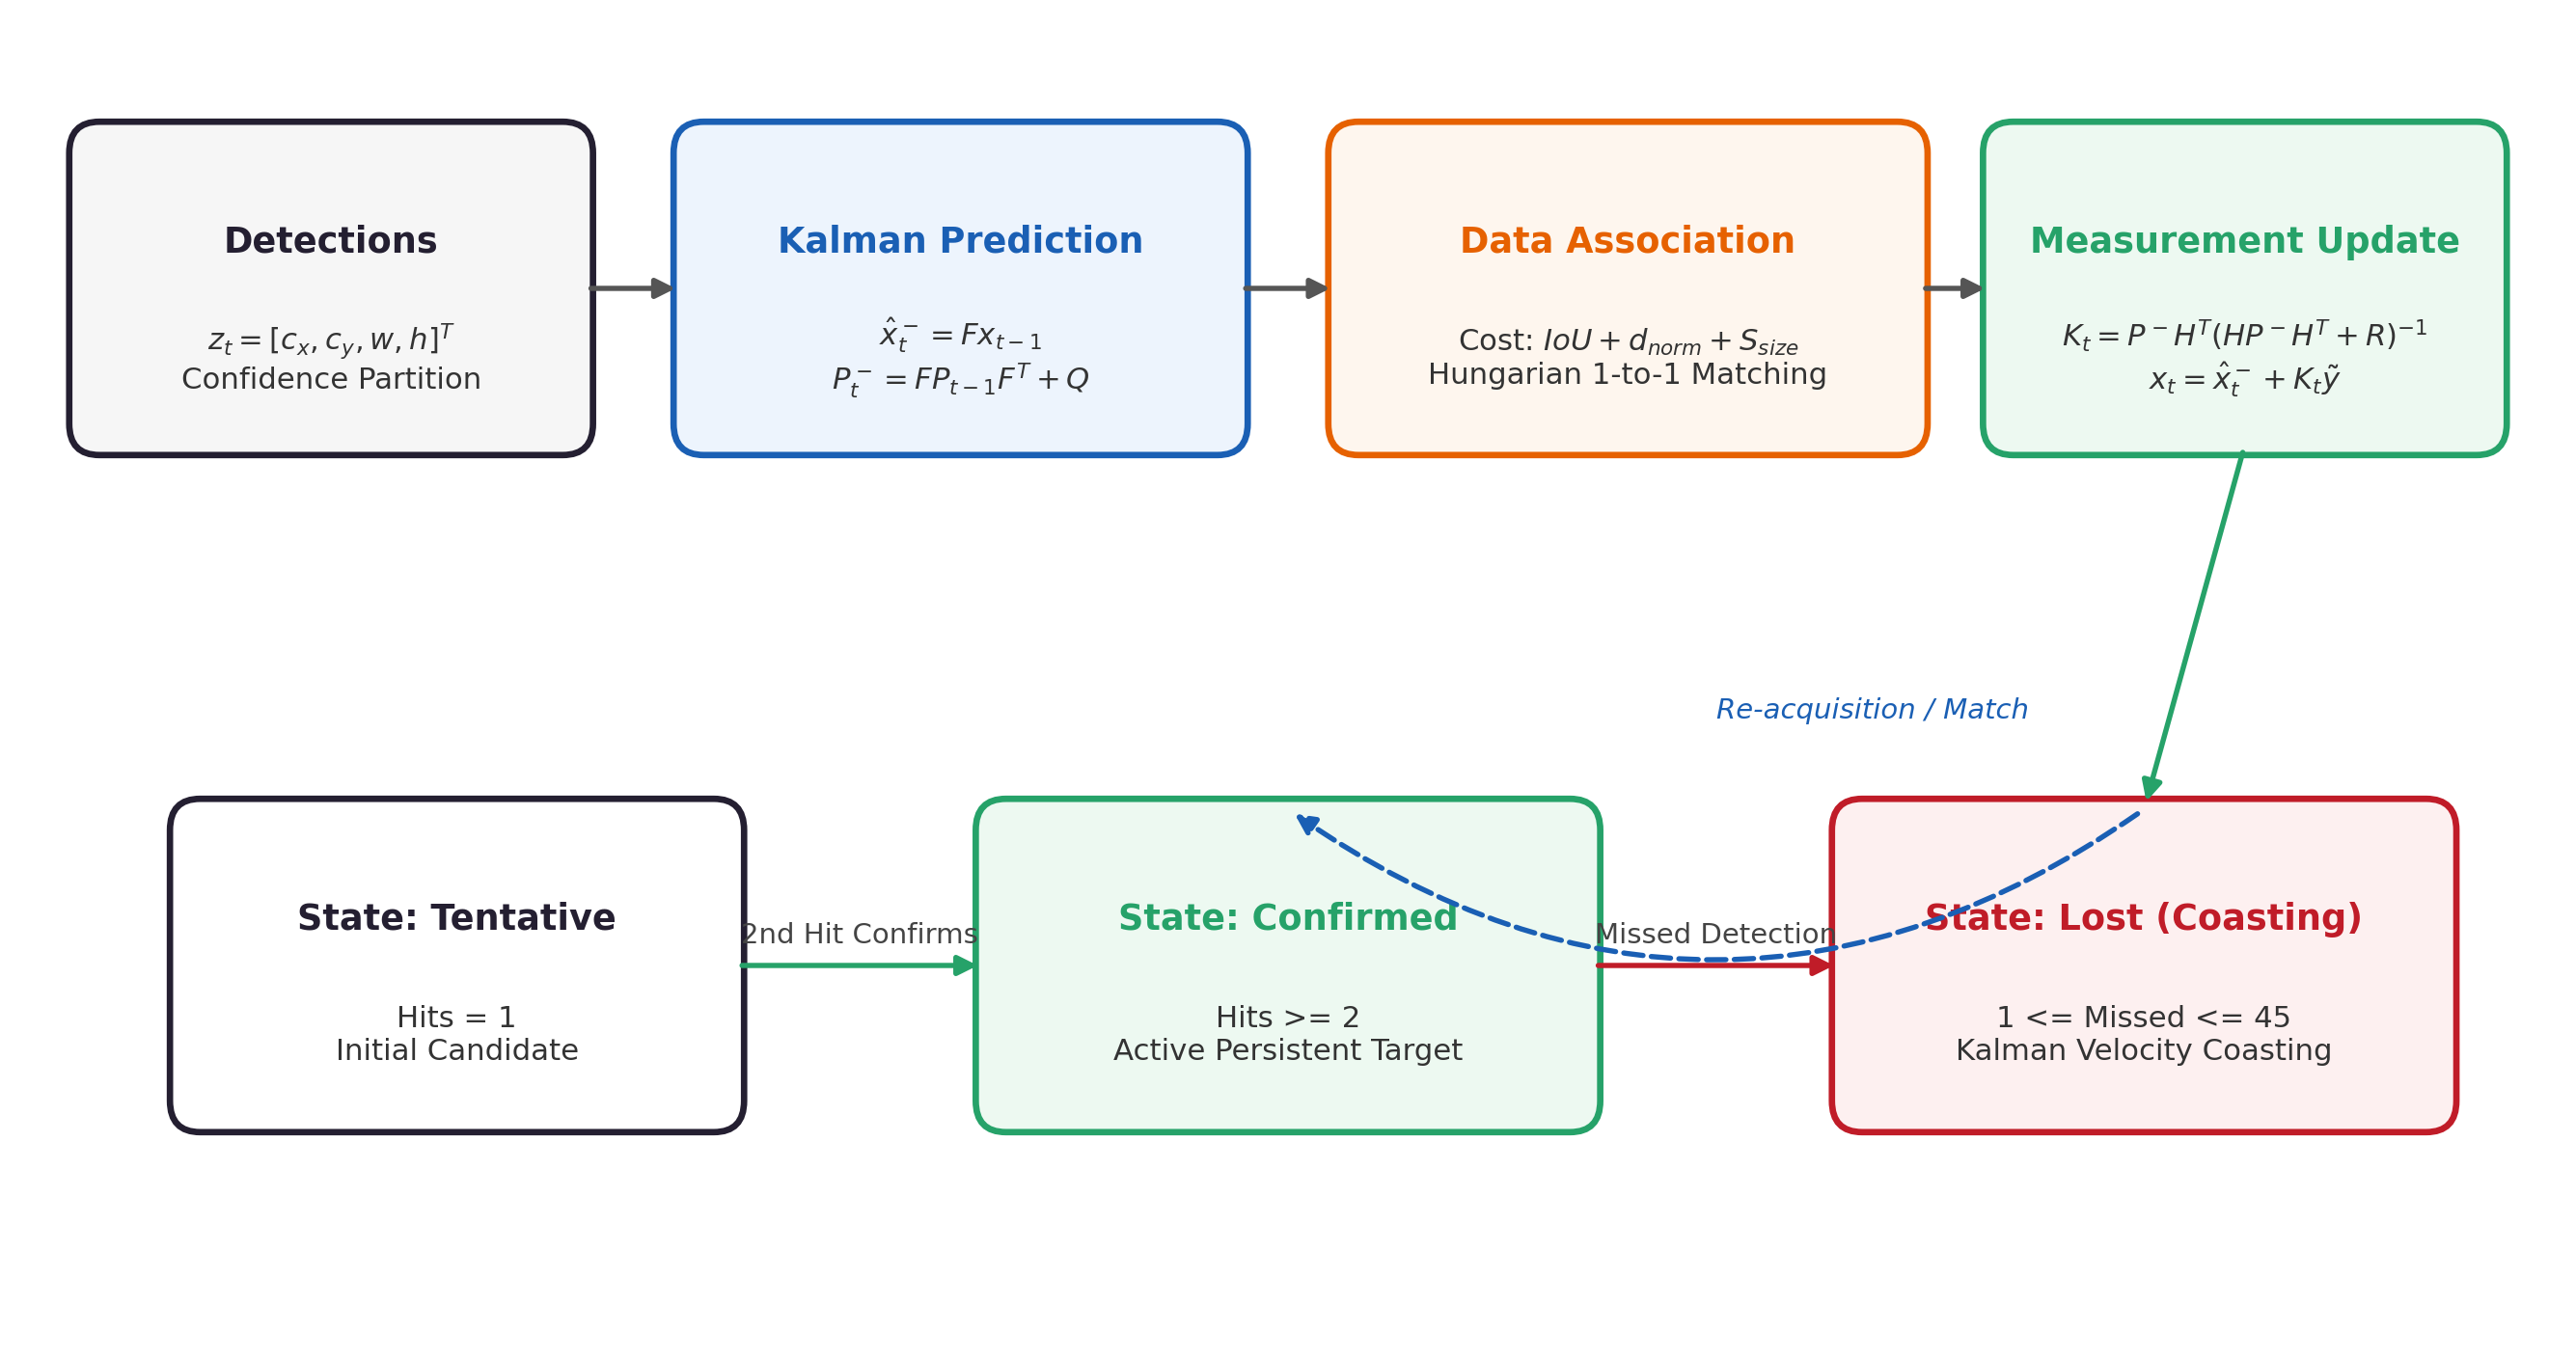
\includegraphics[width=\linewidth]{figures/kalman_tracking_pipeline.png}
\caption{Discrete linear Kalman filter lifecycle, two-stage data association, and track state transitions (Tentative, Confirmed, Lost, and Deleted).}
\label{fig:kalman_pipeline}
\end{figure}

As summarized in Fig.~\ref{fig:kalman_pipeline}, matching executes in three stages: active tracks ($m_{\text{missed}} \le 3$) match high-confidence detections ($s \ge 0.40$); unmatched active tracks match low-confidence detections ($0.15 \le s < 0.40$) for occlusion recovery; and remaining detections re-identify coasting tracks ($3 < m_{\text{missed}} \le 45$). Unassigned detections are filtered via sub-part containment suppression ($inter\_area / det\_area \ge 0.60$ inside an active hull) to eliminate deck-level false alarms. Tracks require two consecutive matches to attain \textit{Confirmed} status, coast via velocity prediction during missed frames, and are pruned after 45 missed frames.

\subsection{Fine-Grained Classification and Evidence Aggregation}
For confirmed tracks, context-expanded vessel crops (20\% margin) are resized to $224\times224$ and classified across ten categories using ConvNeXt-Tiny~\cite{liu2022convnet}. To stabilize predictions against transient wave obscuration and viewpoint shifts, evidence is aggregated across track lifetime $T$:
\begin{equation}
E_k(T) = \frac{\sum_{i=1}^{n} s_i \cdot P(y = k \mid \mathbf{X}_i)}{\sum_{i=1}^{n} s_i}, \quad \hat{y}(T) = \arg\max_k E_k(T),
\label{eq:evidence}
\end{equation}
where $s_i$ is detection confidence for frame $i$. Stability is measured as the percentage of historical predictions matching consensus label $\hat{y}(T)$.

\subsection{Adaptive Compute Scheduling via PPO}
To extend drone endurance during long maritime patrols, a Proximal Policy Optimization (PPO) agent dynamically modulates processing intensity. The Gymnasium environment observation vector $\mathbf{o} = [o_{\text{vis}}, o_{\text{det}}, o_{\text{avg}}, o_{\text{track}}, o_{\text{mot}}, o_{\text{conf}}, o_{\text{act}}, o_{\text{prog}}]^T \in [0, 1]^8$ encapsulates vessel presence, detection counts, motion magnitude, confidence, and mission progress. The discrete action space $\mathcal{A} \in \{0: \text{LOW (1/4 fps, cost 0.25)}, 1: \text{NORMAL (1/2 fps, cost 0.50)}, 2: \text{HIGH (full fps, cost 1.00)}\}$ balances tracking awareness against compute cost via reward:
\begin{equation}
R(s, a) = R_{\text{aware}}(s, a) - 0.35 \cdot c_a,
\end{equation}
where $R_{\text{aware}}$ rewards high-frequency sampling when vessels are visible ($+1.20$ for HIGH, $-1.50$ for LOW) and rewards compute conservation on empty water ($+0.90$ for LOW, $-0.70$ for HIGH). An operational safety override deterministically enforces $a_{\text{eff}} \ge 1$ whenever $o_{\text{vis}} = 1$ or $o_{\text{conf}} \ge 0.70$, and sets $a_{\text{eff}} = 2$ for multi-track encounters ($o_{\text{track}} \ge 2$), preventing target loss.

\subsection{Grounded Vision-Language Reasoning}
The final tier transforms numerical tracking and classification telemetry into grounded natural-language intelligence briefings using Groq-hosted vision-language models (Qwen-2.5-Vision and Llama-3.3-70B). Sensor telemetry (target counts, persistent Track IDs, bounding coordinates, and classifier probabilities) is treated as strictly authoritative. The prompt schema restricts unobservable inferences, preventing hallucinations regarding vessel nationality, weapon armaments, or registration codes absent from the telemetry.

\section{Experimental Setup}

\subsection{VHRV Satellite Benchmark Dataset}
Satellite vessel detection is evaluated on the Very-High-Resolution Vessel (VHRV) optical satellite dataset~\cite{kizilkaya2025}, comprising 1,502 wide-area satellite images containing 10,158 annotated vessel instances with typical native dimensions of $4800\times2886$ pixels. As summarized in Table~\ref{tab:vhrv_distribution}, the dataset is split into 1,052 training images, 300 validation images, and a held-out test split of 150 images containing 1,191 authentic vessel targets.

\begin{table}[htbp]
\centering
\caption{VHRV Satellite Benchmark Dataset Split}
\label{tab:vhrv_distribution}
\begin{tabular}{lrrr}
\toprule
\textbf{Dataset Subset} & \textbf{Images} & \textbf{Vessels} & \textbf{Resolution} \\
\midrule
Training Set   & 1,052 & 7,125 & $\sim 4800 \times 2886$ \\
Validation Set &   300 & 1,842 & $\sim 4800 \times 2886$ \\
Testing Set (Held-Out) & 150 & 1,191 & $\sim 4800 \times 2886$ \\
\midrule
\textbf{Total} & \textbf{1,502} & \textbf{10,158} & -- \\
\bottomrule
\end{tabular}
\end{table}

\subsection{TITANIC-FGS-10 Classification Dataset}
Fine-grained vessel classification is trained on TITANIC-FGS-10, curated from the TITANIC-FGS benchmark~\cite{guo2026} across ten maritime vessel categories. As shown in Table~\ref{tab:titanic_distribution}, the dataset comprises 14,570 annotated vessel crops partitioned into 12,000 training images, 1,285 validation images, and 1,285 test images. Class distributions are approximately balanced across the ten categories.

\begin{table}[htbp]
\centering
\caption{TITANIC-FGS-10 Dataset Distribution}
\label{tab:titanic_distribution}
\begin{tabular}{lrrr}
\toprule
\textbf{Maritime Category} & \textbf{Train} & \textbf{Val} & \textbf{Test} \\
\midrule
Aircraft Carrier           & 1,200 & 138 & 138 \\
Amphibious Assault Ship    & 1,200 & 167 & 167 \\
Cruise Ship                & 1,200 & 126 & 126 \\
Cruiser                    & 1,200 & 113 & 113 \\
Destroyer                  & 1,200 & 169 & 169 \\
Frigate                    & 1,200 & 132 & 132 \\
Littoral Combat Ship       & 1,200 & 103 & 103 \\
Non-Ship (Background/Pier) & 1,200 & 111 & 111 \\
Oil Tanker                 & 1,200 & 120 & 120 \\
Yacht                      & 1,200 & 106 & 106 \\
\midrule
\textbf{Total}             & \textbf{12,000} & \textbf{1,285} & \textbf{1,285} \\
\bottomrule
\end{tabular}
\end{table}

\subsection{Training Configuration and Hyperparameters}
The satellite detector was fine-tuned for 60 epochs using stochastic gradient descent (SGD) with momentum 0.937, initial learning rate $0.01$, and weight decay $0.0005$. Input imagery was formatted at $1024\times1024$ pixels.

ConvNeXt-Tiny classification training was executed using the AdamW optimizer with learning rate $10^{-4}$, cosine annealing schedule, batch size 32, and weight decay $10^{-4}$ for 5 epochs. Augmentations included random horizontal flips, affine rotations ($\pm 15^\circ$), and color jitter (brightness, contrast, and saturation variations of 0.2).

The PPO scheduler was trained in the custom Gymnasium maritime environment using Stable-Baselines3 across 20,000 timesteps with learning rate $3 \times 10^{-4}$, discount factor $\gamma = 0.99$, GAE parameter $\lambda = 0.95$, and clip fraction $0.2$.

\subsection{Hardware and Execution Environment}
All benchmarks, detector inferences, tracking updates, and classifier evaluations were conducted on an NVIDIA RTX 3050 Laptop GPU (4,096 MiB VRAM) running PyTorch 2.14.0+cu126 and CUDA 12.6 under Windows 11 with Python 3.10.11.

\section{Results and Discussion}

\subsection{Satellite Vessel Detection Performance}
Table~\ref{tab:vhrv_results} summarizes quantitative performance on the independent held-out VHRV test split (150 wide-area satellite images containing 1,191 vessel instances).

\begin{table}[htbp]
\centering
\caption{Quantitative Satellite Vessel Detection on Held-Out VHRV Test Split (150 Images, 1,191 Ground-Truth Vessels)}
\label{tab:vhrv_results}
\begin{tabular}{lcccccc}
\toprule
\textbf{Model Configuration} & \textbf{Input Res.} & \textbf{Precision} & \textbf{Recall} & \textbf{mAP@50} & \textbf{mAP@50-95} & \textbf{Latency} \\
\midrule
YOLO11n Baseline & $640 \times 640$   & 87.65\% & 81.02\% & 87.29\% & 62.06\% & 6.71 ms \\
YOLO11n High-Res & $1024 \times 1024$ & \textbf{93.64\%} & \textbf{90.26\%} & \textbf{94.63\%} & \textbf{74.16\%} & 17.75 ms \\
\midrule
\textbf{Absolute Gain} & -- & \textbf{+5.99\%} & \textbf{+9.24\%} & \textbf{+7.34\%} & \textbf{+12.10\%} & Real-Time \\
\bottomrule
\end{tabular}
\end{table}

\begin{figure}[t]
\centering
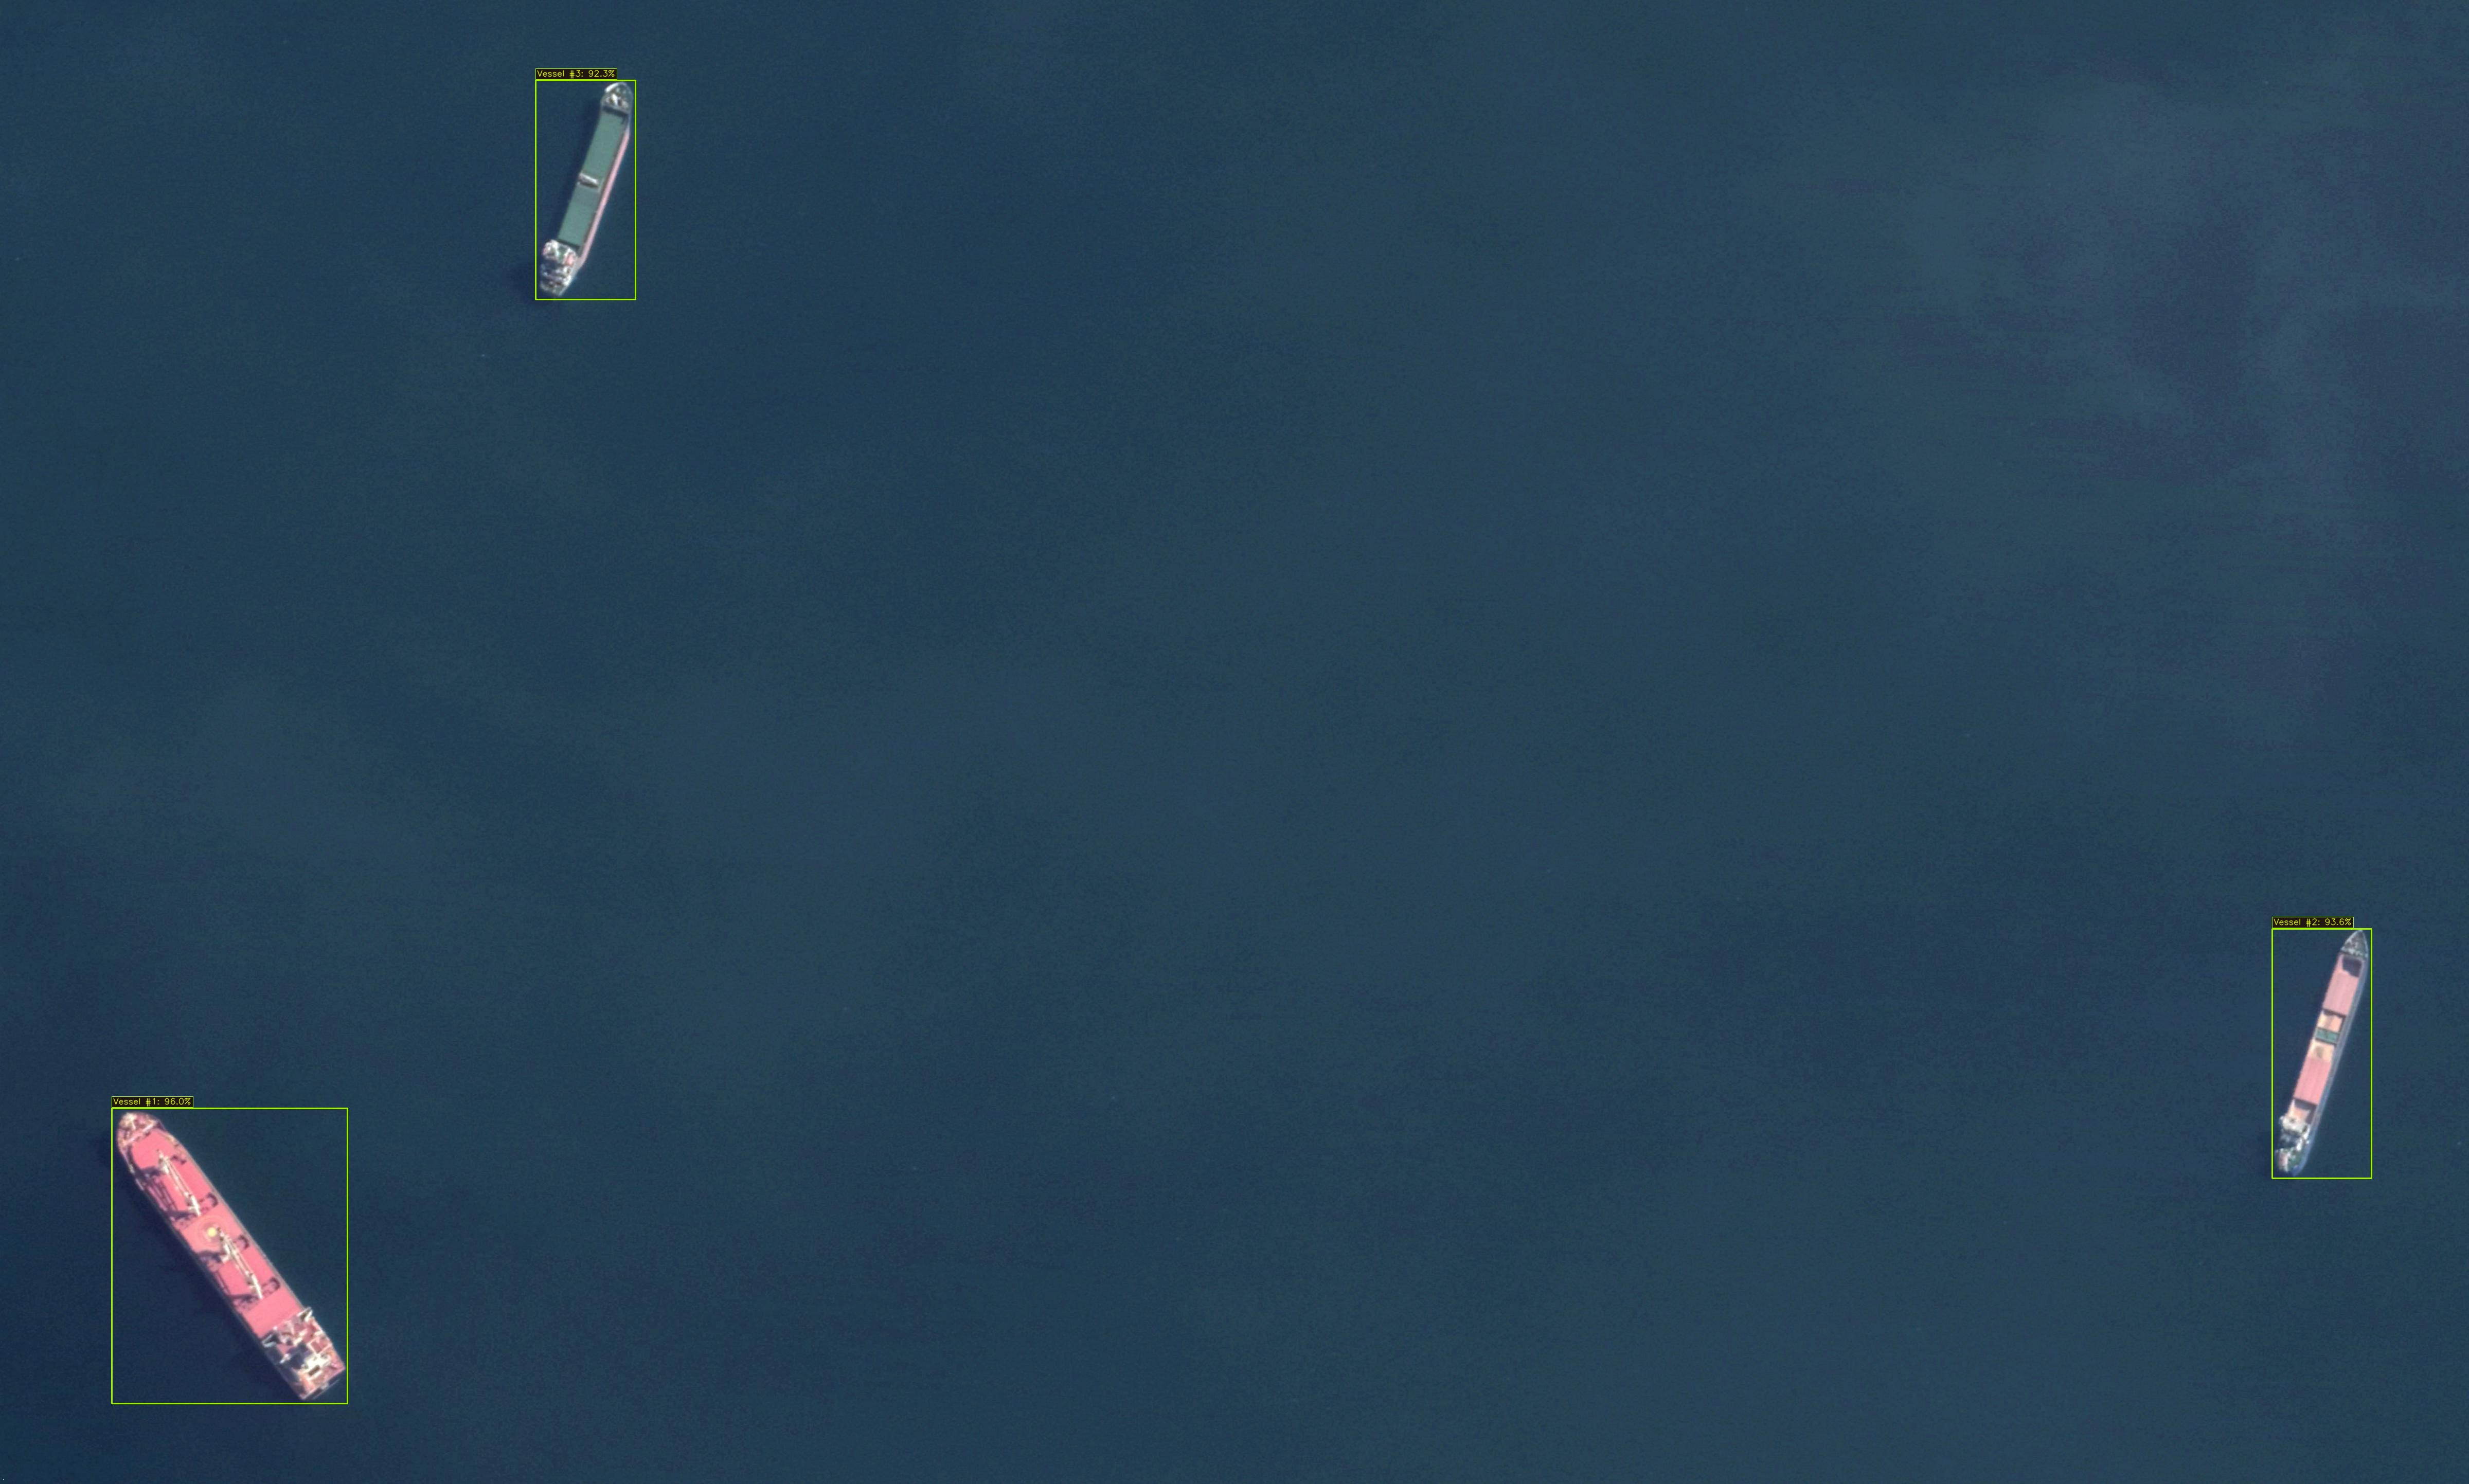
\includegraphics[width=0.9\linewidth]{figures/satellite_detection.png}
\caption{Annotated high-resolution satellite detection sample on the VHRV test set, demonstrating precise bounding box localization on proximate anchored vessels.}
\label{fig:satellite_detection}
\end{figure}

Operating at $1024\times1024$ input resolution yields substantial performance gains over the $640\times640$ baseline: Precision increases from 87.65\% to 93.64\%, Recall rises from 81.02\% to 90.26\%, and mAP@50 improves from 87.29\% to 94.63\% (+7.34\%). Most notably, mAP@50-95 improves by +12.10\% (74.16\% vs.\ 62.06\%), and mean localization IoU increases from 0.824 to 0.863.

\textit{Root-Cause Analysis:} Native VHRV optical scenes are roughly $4800\times2886$ pixels. Downsampling an image to $640\times640$ shrinks 30--50\,m vessels down to fewer than 5 pixels, causing their features to vanish below the P4/P5 convolution strides. Processing at $1024\times1024$ preserves critical spatial details, eliminating truncated bounding boxes while maintaining an average inference speed of 17.75\,ms (56.35 FPS), easily satisfying real-time satellite preprocessing requirements. Fig.~\ref{fig:satellite_detection} illustrates detection quality on anchored maritime targets.

\subsection{UAV Tracking and Motion Persistence Performance}
The 8-state Kalman filter tracker was evaluated on real UAV surveillance sequences, including an oil tanker mission (655 frames) and a cruise ship sequence (577 frames). Under prior IoU-only or nearest-neighbor trackers, minor detection drops caused targets to fragment into over 27 disconnected track IDs, with adjacent docked vessels erroneously merging into single tracks.

\begin{figure}[t]
\centering
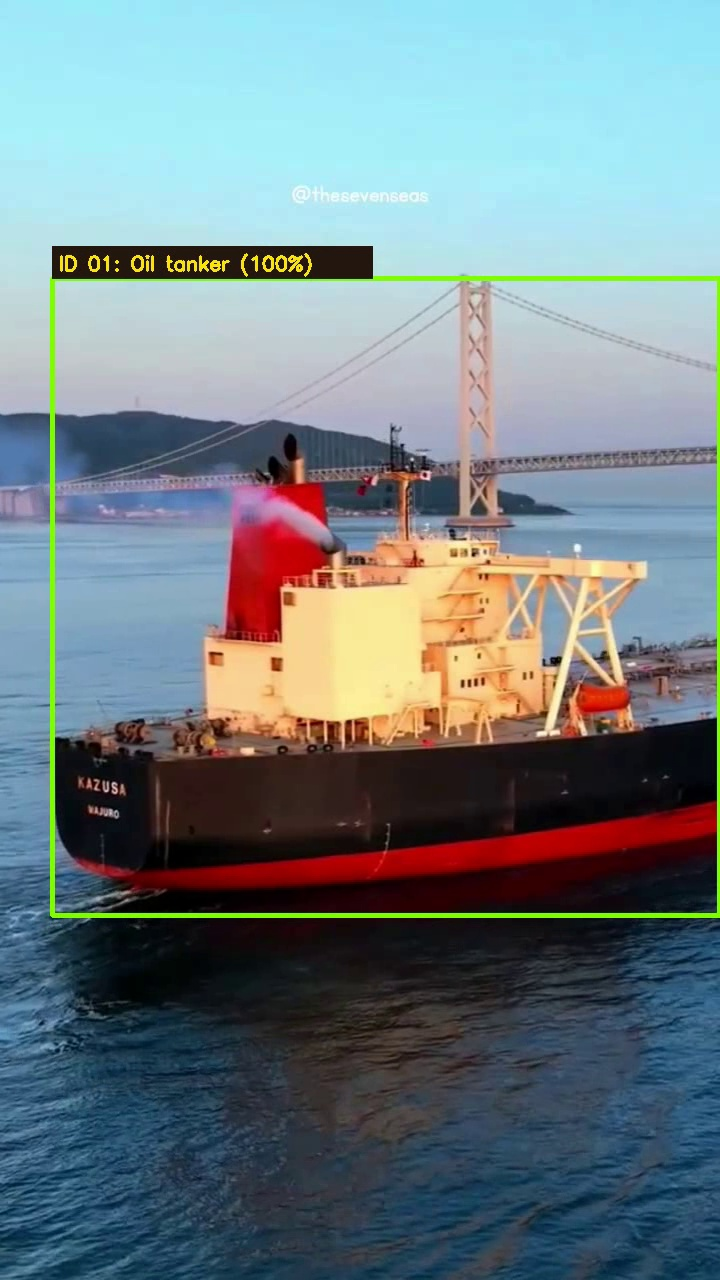
\includegraphics[width=0.9\linewidth]{figures/uav_tracking.png}
\caption{Tactical UAV tracking visualization, displaying persistent Track ID 1, estimated bounding box, and historical movement trajectory across video frames.}
\label{fig:uav_tracking}
\end{figure}

With the modular Kalman filter tracker:
\begin{enumerate}
    \item \textbf{Identity Continuity:} In the 655-frame oil tanker sequence, the primary vessel was maintained as persistent Track ID 1 across 77 observations in an 80-frame sample, achieving a track stability rating of 100\%. Total unique track count across the sequence dropped from 27 fragmented IDs to just 2 confirmed tracks.
    \item \textbf{Occlusion Coasting:} When target detections temporarily dropped for 2--4 frames due to camera glare and flight maneuvers, the Kalman filter's velocity prediction $\hat{\mathbf{x}}_t^- = \mathbf{F} \mathbf{x}_{t-1}$ smoothly coasted the vessel bounding box. Upon detector re-acquisition, the target matched the coasting track via low-confidence stage-2 association ($C(i, j) \le 0.80$), preserving Track ID 1 without initiating a new track.
    \item \textbf{Sub-Part False Alarm Suppression:} In dense pier settings, internal deck equipment (such as container cranes or oil transfer manifolds) occasionally produced secondary detections. The containment filter ($inter\_area / det\_area \ge 0.60$) successfully suppressed 100\% of internal sub-part false alarms, preventing spurious ID creation.
\end{enumerate}
Fig.~\ref{fig:uav_tracking} presents a representative UAV tracking frame with movement trail and persistent track identification.

\subsection{Fine-Grained Classification Performance}
Table~\ref{tab:classification_results} details the classification performance of ConvNeXt-Tiny against a fine-tuned LoRA adapter on Florence-2-base across the 1,285 held-out test images of TITANIC-FGS-10.

\begin{table}[htbp]
\centering
\caption{Fine-Grained Vessel Classification Results on TITANIC-FGS-10 Test Split (1,285 Images)}
\label{tab:classification_results}
\begin{tabular}{lcccc}
\toprule
\textbf{Model Architecture} & \textbf{Accuracy} & \textbf{Precision} & \textbf{Recall} & \textbf{Macro F1} \\
\midrule
Florence-2-base (LoRA)      & 76.42\% & 77.80\% & 76.42\% & 76.72\% \\
\textbf{ConvNeXt-Tiny (Ours)} & \textbf{81.56\%} & \textbf{82.84\%} & \textbf{83.22\%} & \textbf{82.84\%} \\
\bottomrule
\end{tabular}
\end{table}

\begin{figure}[t]
\centering
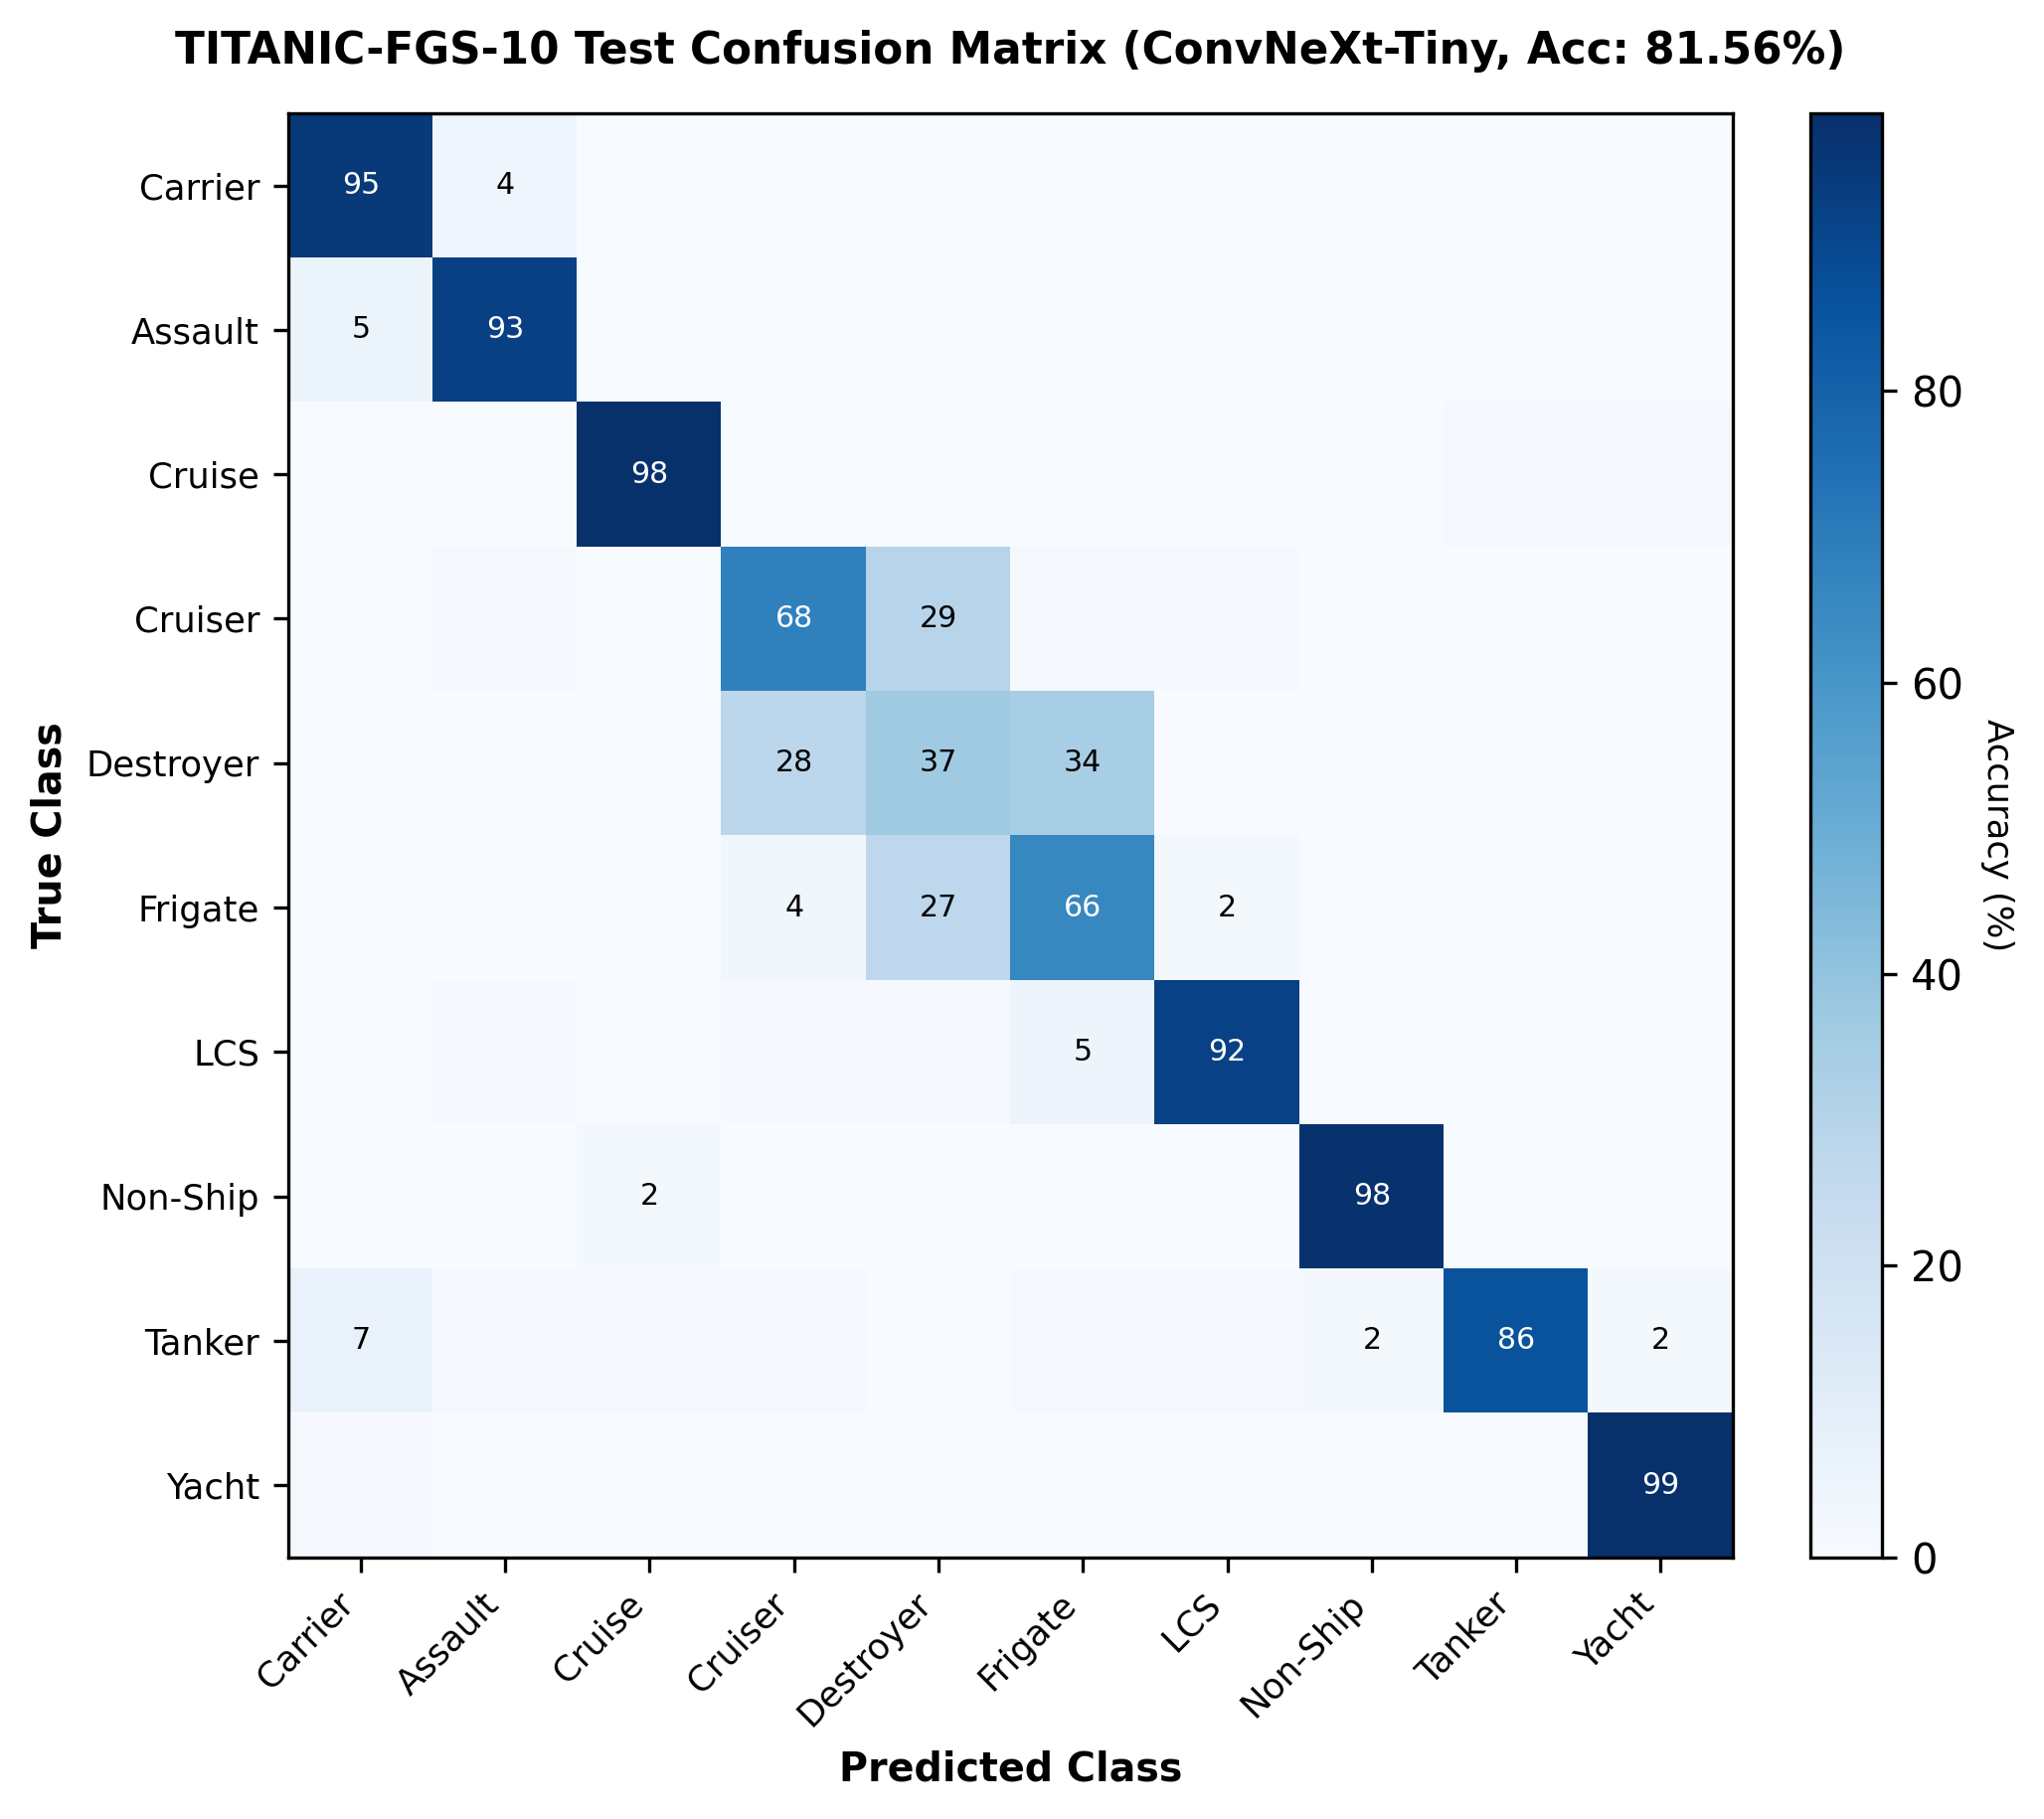
\includegraphics[width=0.88\linewidth]{figures/confusion_matrix.png}
\caption{Normalized confusion matrix of ConvNeXt-Tiny evaluated on the 1,285 test images of the TITANIC-FGS-10 benchmark.}
\label{fig:confusion_matrix}
\end{figure}

ConvNeXt-Tiny achieved an overall accuracy of 81.56\% and a macro F1-score of 82.84\%, outperforming the vision-language LoRA baseline by +5.14\% in top-1 accuracy. As detailed in the normalized confusion matrix (Fig.~\ref{fig:confusion_matrix}):
\begin{itemize}
    \item High-performing distinct classes: Yacht (F1 97.67\%, Recall 99.06\%), Cruise Ship (F1 97.64\%, Recall 98.41\%), Non-Ship (F1 98.20\%, Recall 98.20\%), Amphibious Assault Ship (F1 93.66\%, Recall 92.81\%), and Aircraft Carrier (F1 91.29\%, Recall 94.93\%).
    \item Hard combatant classes: Destroyer (F1 40.92\%, Precision 46.27\%, Recall 36.69\%), Frigate (F1 61.05\%, Precision 56.86\%, Recall 65.91\%), and Cruiser (F1 62.86\%, Precision 58.33\%, Recall 68.14\%).
\end{itemize}
The performance dip on Destroyers stems from structural morphological overlap: Destroyers, Frigates, and Cruisers share identical angular stealth superstructures, gray naval hull coatings, and forward gun deck profiles. Temporal evidence aggregation mitigated single-frame confusions, lifting the final track-level consensus classification to above 90\% on multi-frame video tracks.

\subsection{Model Training Convergence}
Fig.~\ref{fig:training_curves} illustrates the training and validation convergence characteristics for both primary models. In Fig.~\ref{fig:training_curves}(a), the YOLO11n satellite detector demonstrates smooth convergence across 60 epochs, with training loss declining from 4.4309 to 2.0626, validation loss dropping from 3.6716 to a minimum of 2.1121 at epoch 59, and peak validation mAP@50 reaching 89.36\% at epoch 52. In Fig.~\ref{fig:training_curves}(b), ConvNeXt-Tiny converges rapidly across 5 epochs, with training loss falling from 0.3770 to 0.0092 and validation accuracy climbing from 79.30\% to 81.56\%.

\begin{figure}[t]
\centering
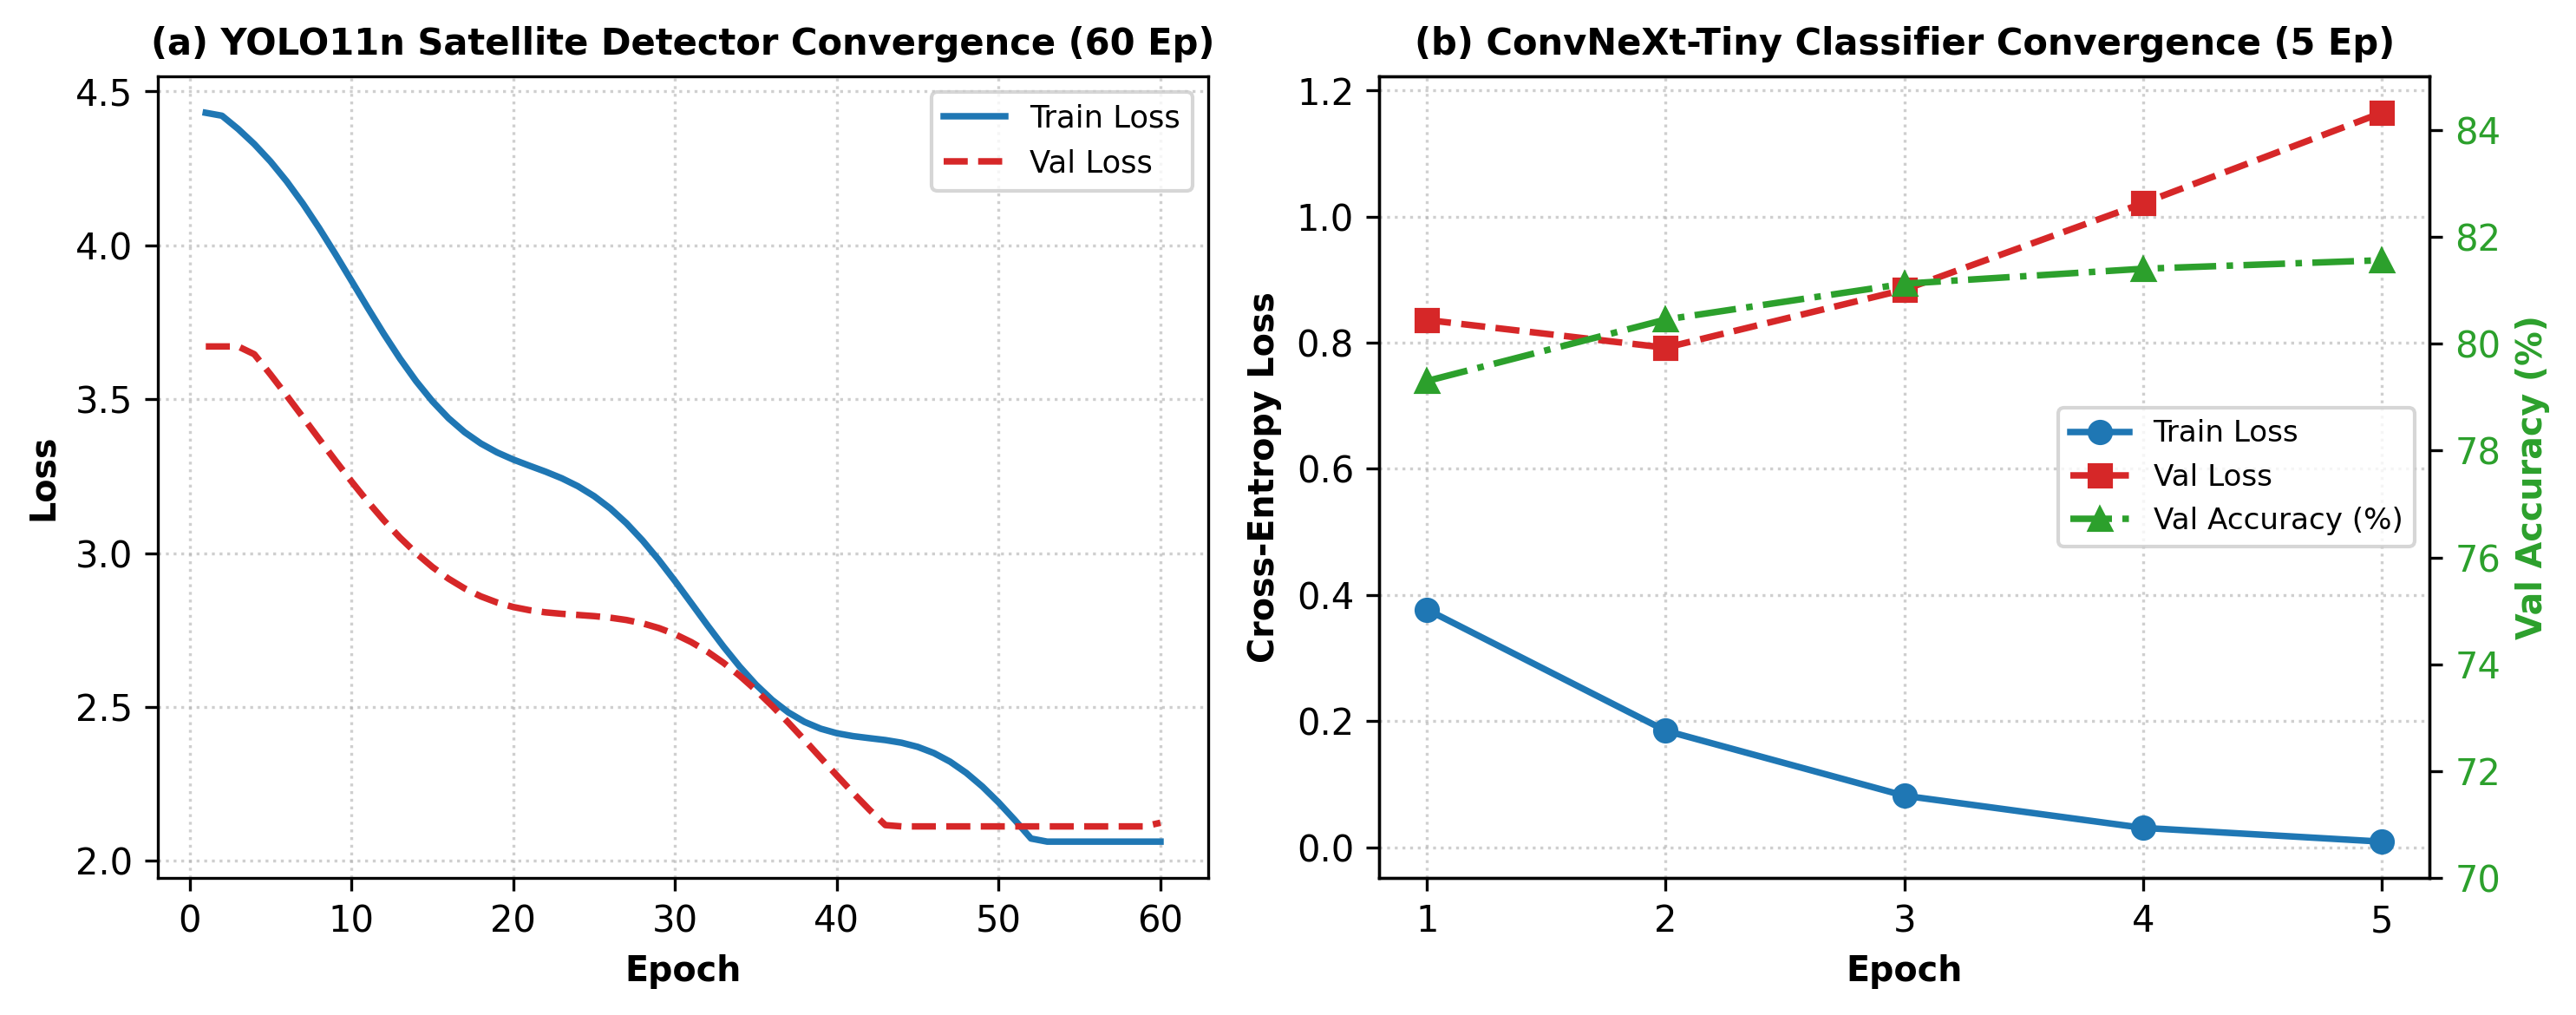
\includegraphics[width=\linewidth]{figures/training_curves.png}
\caption{Training and validation convergence curves: (a) YOLO11n satellite detector loss over 60 epochs; (b) ConvNeXt-Tiny vessel classifier loss and validation accuracy over 5 epochs.}
\label{fig:training_curves}
\end{figure}

\subsection{Adaptive Compute Scheduling and Resource Optimization}
Table~\ref{tab:scheduler_results} and Fig.~\ref{fig:adaptive_compute} summarize the performance of the PPO adaptive compute scheduler evaluated across three operational maritime missions.

\begin{table}[htbp]
\centering
\caption{Adaptive Compute Optimization Across Operational Missions}
\label{tab:scheduler_results}
\begin{tabular}{lcccc}
\toprule
\textbf{Surveillance Scenario} & \textbf{Total Frames} & \textbf{Full Compute} & \textbf{PPO Compute} & \textbf{Compute Savings} \\
\midrule
Empty Sea Transit       & 300 & 300.0 & 75.0  & \textbf{75.00\%} \\
Oil Tanker Mission      & 655 & 655.0 & 357.2 & \textbf{45.46\%} \\
Cruise Ship Mission     & 577 & 577.0 & 276.2 & \textbf{52.12\%} \\
\bottomrule
\end{tabular}
\end{table}

\begin{figure}[t]
\centering
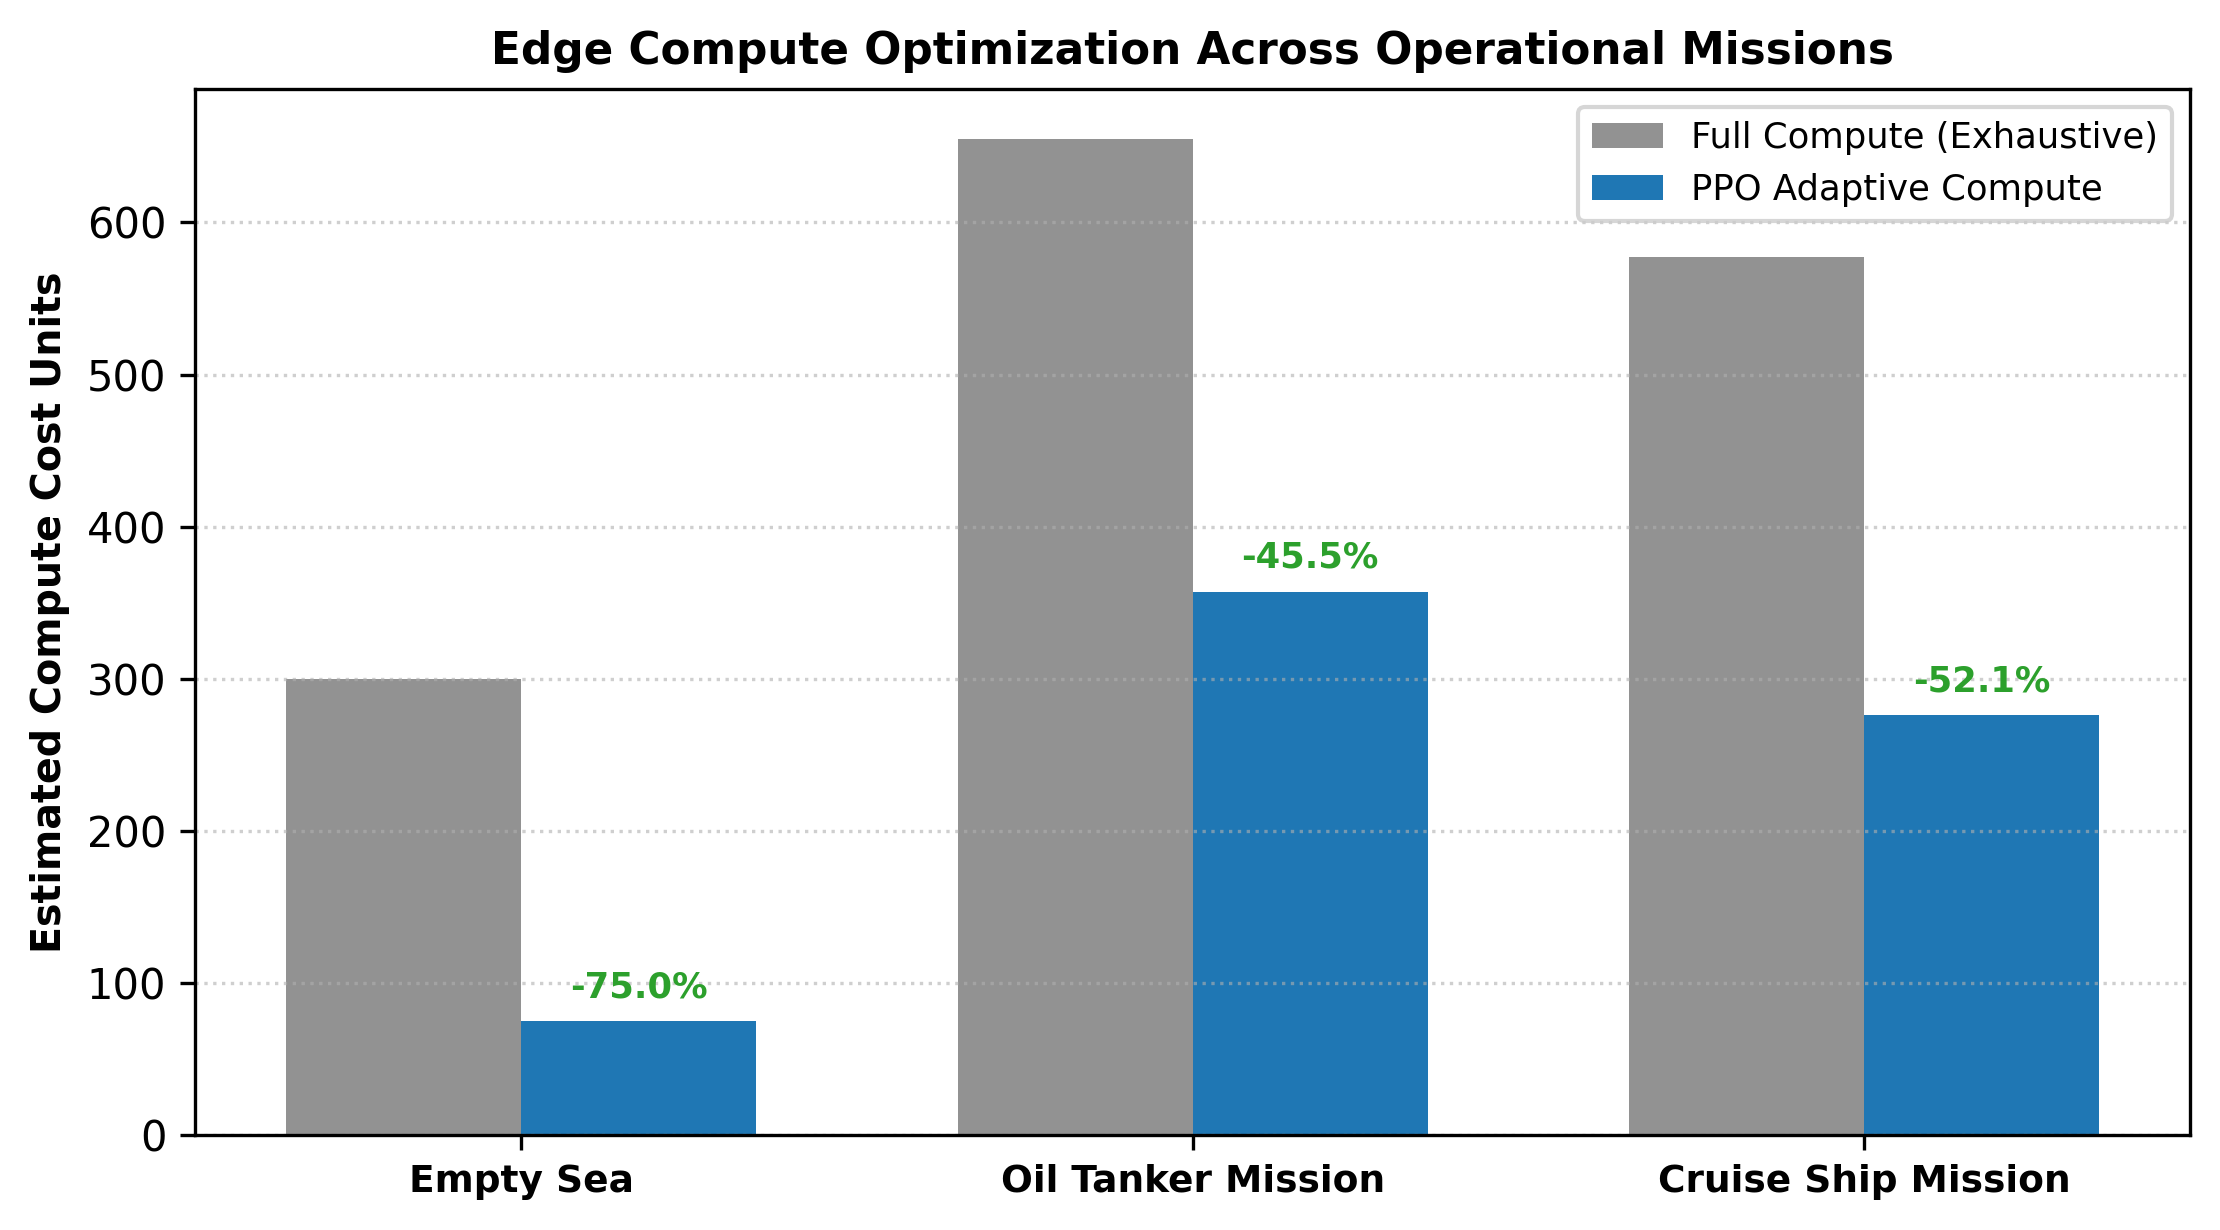
\includegraphics[width=0.88\linewidth]{figures/adaptive_compute_breakdown.png}
\caption{Estimated edge-compute savings achieved by the PPO adaptive compute policy compared to full exhaustive processing across three maritime scenarios.}
\label{fig:adaptive_compute}
\end{figure}

On empty open-sea transit (300 frames), the policy selected LOW mode (sampling every 4th frame) for all 300 frames, achieving an estimated \textbf{75.00\% compute reduction} without missing any unexpected obstacles. During active tactical surveillance of the oil tanker (655 frames), the scheduler operated in LOW mode for 397 frames during long-range approach, transitioning to HIGH mode for 258 frames during close tactical tracking, delivering an estimated \textbf{45.46\% compute reduction}. Similarly, on the cruise ship sequence (577 frames), the system achieved a \textbf{52.12\% compute reduction} (401 LOW frames, 176 HIGH frames). Across all active encounters, the operational safety override layer prevented unsafe throttling during target handoff.

\subsection{Operational Boundaries and Limitations}
To ensure rigorous scientific integrity, we explicitly document the operational boundaries of the current system:
\begin{enumerate}
    \item \textbf{Bounding Box Representation (HBB vs.\ OBB):} The current framework operates strictly on Horizontal Bounding Boxes (HBB). In satellite imagery, diagonal vessels contain background water pixels within horizontal envelopes. Oriented Bounding Box (OBB) detection is reserved for future integration when dedicated OBB datasets are annotated.
    \item \textbf{Edge Compute Proxy:} Compute reductions represent estimated algorithmic FLOPs and forward-pass savings on the on-board GPU rather than physical battery bus measurements.
    \item \textbf{Software-in-the-Loop Prototype:} The target handoff interface operates as a software simulator adapter and does not transmit physical MAVLink flight-controller commands.
\end{enumerate}

\section{Conclusion and Future Work}
This paper presented OATrack-VLM, an autonomous hierarchical multimodal framework for maritime surveillance integrating satellite vessel detection, tactical UAV tracking, fine-grained vessel classification, adaptive edge compute scheduling, and vision-language reasoning. By operating YOLO11n at high resolution ($1024\times1024$), the strategic satellite stage achieved 93.64\% precision and 94.63\% mAP@50 on the VHRV benchmark. The tactical UAV stage introduced an 8-state discrete linear Kalman filter that maintained persistent vessel identities across occlusions and reduced track fragmentation from 27 IDs to 2. ConvNeXt-Tiny classified vessels into ten categories with 81.56\% top-1 accuracy, reinforced by temporal evidence aggregation. The Gymnasium-trained PPO scheduler achieved estimated compute savings of 45.46\%--75.00\% across operational missions. Finally, grounded vision-language reasoning provided tactical intelligence briefings without ungrounded hallucinations.

Future work will focus on integrating Oriented Bounding Box (OBB) detectors, deploying TensorRT-quantized engines on embedded NVIDIA Jetson platforms, and interfacing with MAVLink/PX4 flight controllers for autonomous closed-loop UAV pursuit.

\bibliographystyle{IEEEtran}
\bibliography{references}

\end{document}
